\documentclass[a4paper,11pt]{article}

\usepackage[utf8]{inputenc}

\usepackage{graphicx}
\usepackage{caption}
\usepackage{subcaption}

\usepackage{pgfplots}
\pgfplotsset{compat=1.18} 

\usepackage{minted}
\usepackage{siunitx}

\begin{document}

\title{
    \textbf{Performance of Array Operations in C}
}
\author{Mo Wang}
\date{Spring 2026}

\maketitle

\section*{Introduction}
This report investigates the performance of both linear and binary search algorithm. The primary goal is to analyze the growth of both algorithm's execution time depending on the size of the array. 

\section*{Benchmarking Methodology}

For measuring benchmark execution time, the POSIX monotonic clock (\texttt{CLOCK\_MONOTONIC}) is used by using the helper function \texttt{nano\_seconds()}, which computes the elapsed time in nanoseconds using \texttt{long} integer, given the timestamp pointers \texttt{struct timespec*} \texttt{t\_start} and \texttt{t\_end}.

\begin{minted}[breaklines]{C}
    long nano_seconds(struct timespec *t_start, struct timespec *t_stop) {
        return (t_stop->tv_nsec - t_start->tv_nsec) +
               (t_stop->tv_sec - t_start->tv_sec) * 1000000000;
    }
    // memory allocation for array
    clock_gettime(CLOCK_MONOTONIC, &t_start);
    // algorithm
    clock_gettime(CLOCK_MONOTONIC, &t_stop);
    // deallocate array memory
    return nano_seconds(&t_start, &t_stop);
\end{minted}

However, the precision is typically on the order of hundreds nanoseconds, which makes timing individual operations unreliable. To mitigate this, each algorithm is executed repeatedly in a batch (1024 iterations) to measure the total execution time of the batch. Execution time of each operation can be calculated by dividing the batch execution time by number of iterations.

Due to hardware constraints, operating system scheduling, and background process, execution time can fluctuate between each operation execution. To minimize the uncertainty, each benchmark is repeated multiple times while reporting the minimum elapsed time.

\section*{Linear search algorithm}

\iffalse
Set up the rest of a benchmark and do some measurements for a growing number of elements in the array. Describe the relationship between the size of the array and the time it takes to do the search. How long time does it take to search through an array of a million elements? + Benchmark statistics diagrams, regression and time complexity
sorted linear search: Now, if we know that the array is sorted we can of course do a quick optimization - we can stop the search once the next element in the array is larger then the key that we are looking for. Take a wild guess, how much better is this compared to our unsorted solution? + Benchmark statistics table+diagrams, regression and time complexity
\fi

A linear search algorithm searches for a given key in an unsorted array by starting at the first element and comparing each element to the key one by one. If the element matches the key, the algorithm returns the index of that element. If the end of the array is reached without a match, the key doesn't exist in array and the largest unsigned integer value is returned.

\begin{minted}{c}
  unsigned int linear_search(int array[], unsigned int length, int key) {
      for (int index = 0; index < length; index++) {
          if (array[index] == key) {
              return index;
          }
      }
      return UINT_MAX;
  }
\end{minted}

In terms of elapsed time of the algorithm, the whole array is iterated over in worst case. Given the array size $n$, $n$ amount of comparison checks are performed in worst case. However in best case scenario, the first element matches the key, thus only one comparison is conducted. The estimated average time is calculated as $t(n)=a(1+t)/2=1/2+t/2$, where $a$ is the time cost for number comparison, which falls into $O(n)$ time complexity.

\begin{table}[h]
\begin{center}
\begin{tabular}{l|cccccccc}
\textbf{Size} 
    & 1024 & 2048 & 4096 & 8192 & 16384 & 32768 & 65536 & 131072 \\
\hline
\textbf{ns} 
    & $9.0\times10^{2}$ 
    & $1.8\times10^{3}$ 
    & $3.6\times10^{3}$ 
    & $7.3\times10^{3}$ 
    & $1.4\times10^{4}$ 
    & $2.8\times10^{4}$ 
    & $5.6\times10^{4}$ 
    & $1.1\times10^{5}$ \\
\end{tabular}
\caption{Linear search in an unsorted array: elapsed time per loop (transposed)}
\label{tab:linear-search-transposed}
\end{center}
\end{table}

The benchmark result with its regression also shows the same growth trend where doubling the size roughly doubles the elapsed time.

\begin{figure}[h]
  \centering
  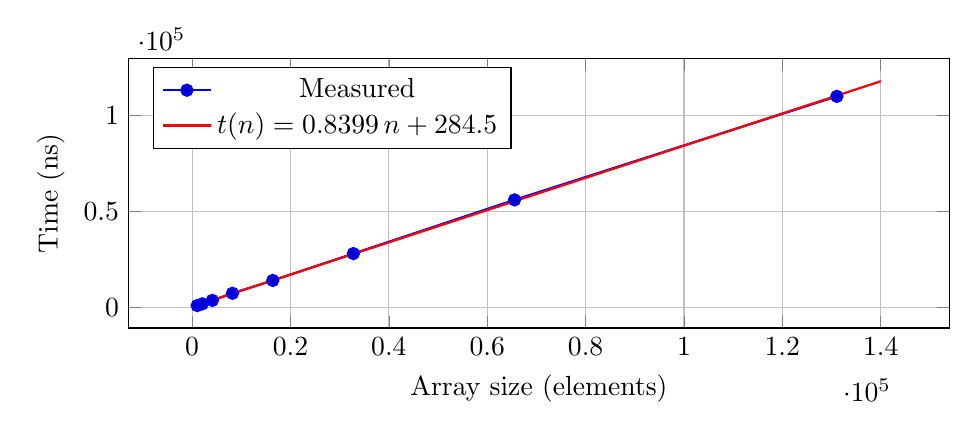
\begin{tikzpicture}
    \begin{axis}[
      xlabel={Array size (elements)},
      ylabel={Time (ns)},
      width=12cm, height=5cm,
      grid=major,
      legend pos=north west,
      ymajorgrids=true,
      xmajorgrids=true
    ]
      % Benchmark data points
      \addplot+[
        mark=*,
        thick,
        color=blue
      ] coordinates {
        (1024,   9.0e2)
        (2048,   1.8e3)
        (4096,   3.6e3)
        (8192,   7.3e3)
        (16384,  1.4e4)
        (32768,  2.8e4)
        (65536,  5.6e4)
        (131072, 1.1e5)
      };
      \addlegendentry{Measured}

      % Least-squares linear fit: t(n) = a*n + b
      % a ≈ 0.8399354126, b ≈ 284.5081332
      \addplot[
        red,
        thick,
        domain=1000:140000,
        samples=200
      ] {0.8399354126*x + 284.5081332};
      \addlegendentry{$t(n) = 0.8399\,n + 284.5$}

    \end{axis}
  \end{tikzpicture}
  \caption{Linear search benchmark with least-squares linear fit}
  \label{fig:linear-search}
\end{figure}

However, given that the array is stored, a quick optimization can be performed by stopping the search once the next element is larger than the key. Despite early exiting array, the algorithm still has linear time complexity, since the array has to be iterated over fully in worst case scenario when key is larger than any element in the array. On the flip side, the coefficients are smaller, causing the time complexity to increase slower as the array size grows, which is shown in Table 2 and Figure 2.

\begin{table}[h]
\begin{center}
\begin{tabular}{l|cccccccc}
\textbf{Size} 
    & 1024 & 2048 & 4096 & 8192 & 16384 & 32768 & 65536 & 131072 \\
\hline
\textbf{ns} 
    & $1.0\times10^{3}$
    & $2.1\times10^{3}$
    & $4.2\times10^{3}$
    & $8.2\times10^{3}$
    & $1.7\times10^{4}$
    & $3.2\times10^{4}$
    & $6.6\times10^{4}$
    & $1.3\times10^{5}$ \\
\end{tabular}
\caption{Linear search in a sorted array: elapsed time per loop (transposed)}
\label{tab:linear-search-sorted-transposed}
\end{center}
\end{table}

\begin{figure}[h]
  \centering
  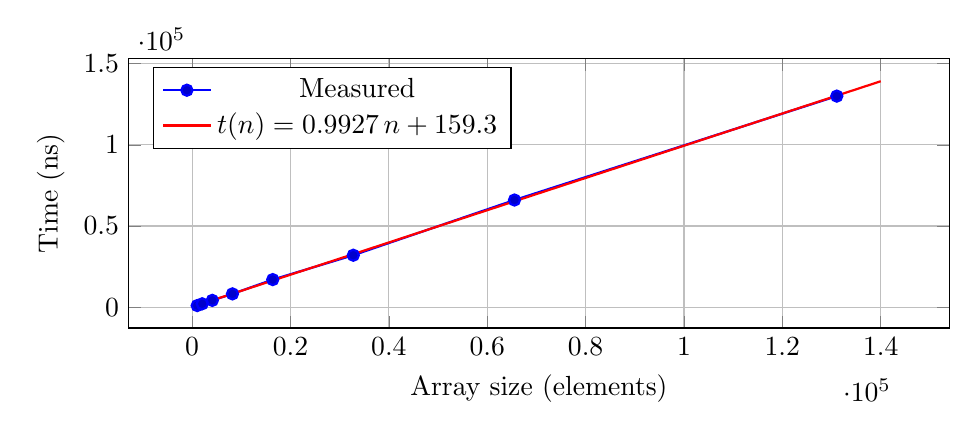
\begin{tikzpicture}
    \begin{axis}[
      xlabel={Array size (elements)},
      ylabel={Time (ns)},
      width=12cm, height=5cm,
      grid=major,
      legend pos=north west,
      ymajorgrids=true,
      xmajorgrids=true
    ]
      % Measured data points
      \addplot+[
        mark=*,
        thick,
        color=blue
      ] coordinates {
        (1024,   1.0e3)
        (2048,   2.1e3)
        (4096,   4.2e3)
        (8192,   8.2e3)
        (16384,  1.7e4)
        (32768,  3.2e4)
        (65536,  6.6e4)
        (131072, 1.3e5)
      };
      \addlegendentry{Measured}

      % Least-squares linear fit: t(n) = a*n + b
      % a ≈ 0.99274406098, b ≈ 159.33384973
      \addplot[
        red,
        thick,
        domain=1000:140000,
        samples=200
      ] {0.99274406098*x + 159.33384973};
      \addlegendentry{$t(n) = 0.9927\,n + 159.3$}

    \end{axis}
  \end{tikzpicture}
  \caption{Linear search in a sorted array with least-squares linear fit}
  \label{fig:linear-search-sorted}
\end{figure}

\section*{Binary search}

\iffalse
How long time does it take to search through an array of a million entries? It might not sound very much but if our program constantly does search operations it will add up. There are however smarter things we can do and this will allow us to handle much larger data sets in reasonable time.

Re-run your benchmarks but now using the binary search. Report the execution time and describe a function that given the size of the array roughly describes the execution time. How long time does it take to search through an array of one million items? Without running an experiment - how long time do you estimate that it would take to search through an array of 64M items? Give it a try- how well did you estimate the execution time?  + Benchmark statistics table+diagrams, regression and time complexity
\fi

On the other hand, a binary search starts in the middle of an array. If the element matches the key, the element is found, while its index is returned. Otherwise, the element is compared to the key and repeat the process in right interval if the key is larger than given element and left if key is smaller. Using this approach, half of the elements are eliminated from searching on each iteration, which means only a fraction of element comparison needs to be performed in the array. Searching $n$ elements in an array, only $log_2(n)$ iteration is required with one element comparison in each iteration that takes $a$ time, which gives time function $t(n)=log_2(n)*a$ in $O(log(n))$ time complexity.

\begin{minted}{c}
  unsigned int binary_search(int array[], unsigned int length, int key) {
      int first = 0;
      int last = length-1;
      while (true) {
          // jump to the middle
          int index = (first + last)/2;
          if (array[index] == key) {
              return index;
          }
          if (array[index] < key && index < last) {
              first = index + 1;
              continue;
          }
          if (array[index] > key && index > first) {
              last = index - 1;
              continue;
          }
          return UINT_MAX;
      }
  }
\end{minted}

\begin{table}[h]
\begin{center}
\begin{tabular}{l|cccccccc}
\textbf{Size}
    & 1024 & 2048 & 4096 & 8192 & 16384 & 32768 & 65536 & 131072 & 1000000 & 64000000 \\
\hline
\textbf{ns}
    & 54
    & 69
    & 73
    & 92
    & 97
    & $1.2\times10^{2}$
    & $1.3\times10^{2}$
    & $1.3\times10^{2}$
    & $2.4\times10^{2}$
    & $1.1\times10^{3}$ \\
\end{tabular}
\caption{Binary search: elapsed time per loop (transposed)}
\label{tab:binary-search-transposed}
\end{center}
\end{table}

Benchmark results show that for 1M data ...

Measured elapsed time using benchmark shows that an array with 1 million elements takes roughly $2.4\times10^2$ ns. Following the same trend, doubling each element adds on 12 ns to elapsed time, which means that for 64 million elements, the elapsed time is roughly $a\cdot log_2(64\cdot 10^6) = a\cdot log_2(10^6)\cdot 6 = 2.4\cdot10^2\cdot 6 = 1.44\cdot 10^3$ ns. The actual measurement for 64 million elements is $1.1\cdot10^3$ ns, which roughly matches the growth trend.

\begin{figure}[h]
  \centering
  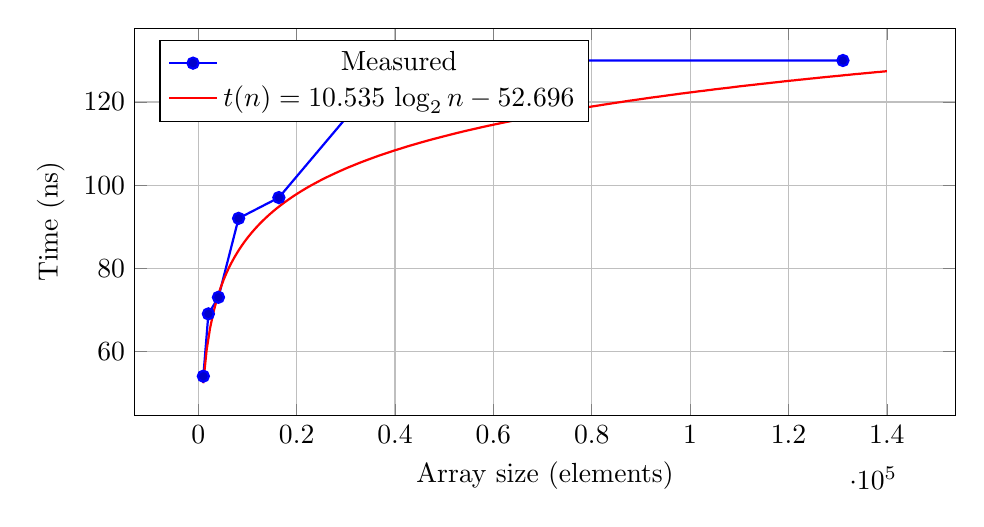
\begin{tikzpicture}
    \begin{axis}[
      xlabel={Array size (elements)},
      ylabel={Time (ns)},
      width=12cm, height=6.5cm,
      grid=major,
      legend pos=north west,
      ymajorgrids=true,
      xmajorgrids=true
    ]

      % Measured data
      \addplot+[
        mark=*,
        thick,
        color=blue
      ] coordinates {
        (1024,   54)
        (2048,   69)
        (4096,   73)
        (8192,   92)
        (16384,  97)
        (32768,  120)
        (65536,  130)
        (131072, 130)
      };
      \addlegendentry{Measured}

      % Fitted curve: t(n) = 10.535 log2(n) - 52.696
      \addplot[
        red,
        thick,
        domain=1000:140000,
        samples=200
      ] {10.535*(ln(x)/ln(2)) - 52.696};
      \addlegendentry{$t(n)=10.535\,\log_2 n - 52.696$}

    \end{axis}
  \end{tikzpicture}
  \caption{Binary search benchmark with $\log_2 n$ least-squares fit}
  \label{fig:binary-search}
\end{figure}



\section*{Recursive binary search}

\iffalse
procedure calls are expensive, using the programming stack extensively
How many recursive calls are done when searching an array or length
1000? How many are done when searching: 2000, 4000 ... a million? Is the number of recursive calls on the stack a problem? + evaluation
+ Benchmark statistics table+diagrams, regression and time complexity
Comparing recursive vs. iterative performance in execution time + table + diagram
Discussing overhead beyond stack depth
\fi

The binary search algorithm can also be implemented using recursion. Every iteration in the while loop is swapped to a recursive function call in recursive implementation, which narrows the search interval until a key is found.

\begin{minted}{c}
  unsigned int recursive_binary_search(
      int array[],
      unsigned int length,
      int key,
      unsigned int first,
      unsigned int last
  ) {
      if (first > last)
          return UINT_MAX;
  
      unsigned int index = (first + last) / 2;
  
      if (array[index] == key)
          return index;
  
      if (array[index] < key)
          return recursive_binary_search(array, length, key, index + 1, last);
  
      return recursive_binary_search(array, length, key, first, index - 1);
  }
  
\end{minted}

The benchmark shows the same logarithmic time growth, since the elapsed time is similar. 

\begin{table}[h]
\begin{center}
\begin{tabular}{l|cccccccc}
\textbf{Size}
    & 1024 & 2048 & 4096 & 8192 & 16384 & 32768 & 65536 & 131072 \\
\hline
\textbf{ns}
    & 56
    & 76
    & 83
    & 94
    & 95
    & $1.1\times10^{2}$
    & $1.3\times10^{2}$
    & $1.4\times10^{2}$ \\
\end{tabular}
\caption{Recursive binary search: elapsed time per loop (transposed)}
\label{tab:recursive-binary-search-transposed}
\end{center}
\end{table}



\section*{Conclusion}

\iffalse
Differences in behavior between unsorted search and sorted search, as well as recursive and iterative performance
\fi

\end{document}
